% Created 2025-10-06 Mon 16:44
% Intended LaTeX compiler: lualatex
\documentclass[a4paper,12pt]{article}
\usepackage{amsmath}
\usepackage{fontspec}
\usepackage{graphicx}
\usepackage{longtable}
\usepackage{wrapfig}
\usepackage{rotating}
\usepackage[normalem]{ulem}
\usepackage{capt-of}
\usepackage{hyperref}
\usepackage{luacode}
\usepackage[english, french]{babel}
\usepackage{microtype}
\usepackage[autolanguage]{numprint}
\npthousandsep{~}
\usepackage{fontspec}
\usepackage{ulem}
\usepackage{soul}
\setmainfont{Source Serif 4}[Path=/home/anthea/org/fonts/Source_Serif_4/static/, UprightFont=SourceSerif4-Regular.ttf, ItalicFont=SourceSerif4-Italic.ttf, BoldFont=SourceSerif4-Bold.ttf, BoldItalicFont=SourceSerif4-BoldItalic.ttf]
\setsansfont{Source Sans 3}[Path=/home/anthea/org/fonts/Source_Sans_3/static/, UprightFont=SourceSans3-Regular.ttf, ItalicFont=SourceSans3-Italic.ttf, BoldFont=SourceSans3-Bold.ttf, BoldItalicFont=SourceSans3-BoldItalic.ttf]
\setmonofont{Source Code Pro}[Path=/home/anthea/org/fonts/Source_Code_Pro/static/, UprightFont=SourceCodePro-Regular.ttf, ItalicFont=SourceCodePro-Italic.ttf, BoldFont=SourceCodePro-Bold.ttf, BoldItalicFont=SourceCodePro-BlackItalic.ttf]
\renewcommand{\familydefault}{\sfdefault}
\renewcommand{\tiny}{\small}
\renewcommand{\scriptsize}{\small}
\usepackage[usenames,dvipsnames,svgnames,table]{xcolor}
\definecolor{customgray}{HTML}{505050}
\usepackage[top=3.2cm, bottom=3.2cm, left=2.4cm, right=2.4cm]{geometry}
\usepackage{setspace,fancyhdr,indentfirst,lastpage,datetime,authblk,ifthen,etoolbox,titling}
\singlespacing
\pagestyle{fancy}
\fancyhf{}
\fancyfoot[C]{\thepage\ / \pageref{LastPage}}
\renewcommand{\headrulewidth}{0pt}
\setlength{\parindent}{0pt}
\setcounter{secnumdepth}{3}
\setlength{\columnsep}{0.8cm}
\setlength{\marginparwidth}{1.6cm}
\setcounter{page}{1}
\usepackage{csquotes}
\usepackage{array,booktabs,multirow,tabularx,colortbl,diagbox,makecell,ltablex,adjustbox,multicol}
\usepackage{enumitem}\setlist{nosep}\setlist[itemize]{leftmargin=*}
\usepackage[toc,page]{appendix}
\usepackage[nottoc]{tocbibind}
\newenvironment{keyword}{\begin{trivlist}\item[]{\bfseries Mots-clés :}}{\end{trivlist}}
\usepackage{graphicx,caption,wrapfig}
\usepackage[most,breakable,xparse,listings,skins]{tcolorbox}
\usepackage[colorinlistoftodos]{todonotes}
\usepackage{newfloat}
\DeclareFloatingEnvironment[fileext=lol,listname={\vspace{-2em}},name=Listing]{listing}
\captionsetup{format=plain,font=small,labelfont=bf}
\captionsetup[listing]{labelfont=bf,textfont=it}
\usepackage{fvextra,amsfonts,amssymb,amsmath,mathrsfs,mathtools,stmaryrd}
\usepackage{algorithm2e}
\usepackage{pgf,tikz,pgfplots,pgfplotstable,arydshln,subcaption,forest}
\pgfplotsset{compat=1.18}
\usepackage[acronym]{glossaries}
\makenoidxglossaries
\usepackage{url,orcidlink,hyperref}
\hypersetup{colorlinks=true, linkcolor=customgray, citecolor=customgray, urlcolor=customgray, pdfborder={0 0 0}, unicode=true}
\setcounter{secnumdepth}{3}
\author{PA156562}
\date{\today}
\title{}
\hypersetup{
 pdfauthor={PA156562},
 pdftitle={},
 pdfkeywords={},
 pdfsubject={},
 pdfcreator={},
 pdflang={French}}

% Setup for code blocks [1/2]

\usepackage{fvextra}

\fvset{%
  commandchars=\\\{\},
  highlightcolor=white!95!black!80!blue,
  breaklines=true,
  breaksymbol=\color{white!60!black}\tiny\ensuremath{\hookrightarrow}}

% Make line numbers smaller and grey.
\renewcommand\theFancyVerbLine{\footnotesize\color{black!40!white}\arabic{FancyVerbLine}}

\usepackage{xcolor}

% In case engrave-faces-latex-gen-preamble has not been run.
\providecolor{EfD}{HTML}{f7f7f7}
\providecolor{EFD}{HTML}{28292e}

% Define a Code environment to prettily wrap the fontified code.
\usepackage[breakable,xparse]{tcolorbox}
\DeclareTColorBox[]{Code}{o}%
{colback=EfD!98!EFD, colframe=EfD!95!EFD,
  fontupper=\footnotesize\setlength{\fboxsep}{0pt},
  colupper=EFD,
  IfNoValueTF={#1}%
  {boxsep=2pt, arc=2.5pt, outer arc=2.5pt,
    boxrule=0.5pt, left=2pt}%
  {boxsep=2.5pt, arc=0pt, outer arc=0pt,
    boxrule=0pt, leftrule=1.5pt, left=0.5pt},
  right=2pt, top=1pt, bottom=0.5pt,
  breakable}

% Support listings with captions
\usepackage{float}
\floatstyle{plain}
\newfloat{listing}{htbp}{lst}
\newcommand{\listingsname}{Listing}
\floatname{listing}{\listingsname}
\newcommand{\listoflistingsname}{List of Listings}
\providecommand{\listoflistings}{\listof{listing}{\listoflistingsname}}


% Setup for code blocks [2/2]: syntax highlighting colors

\newcommand\efstrut{\vrule height 2.1ex depth 0.8ex width 0pt}
\definecolor{EFD}{HTML}{000000}
\definecolor{EfD}{HTML}{ffffff}
\newcommand{\EFD}[1]{\textcolor{EFD}{#1}} % default
\definecolor{EFvp}{HTML}{000000}
\newcommand{\EFvp}[1]{\textcolor{EFvp}{#1}} % variable-pitch
\definecolor{EFh}{HTML}{7f7f7f}
\newcommand{\EFh}[1]{\textcolor{EFh}{#1}} % shadow
\definecolor{EFsc}{HTML}{228b22}
\newcommand{\EFsc}[1]{\textcolor{EFsc}{\textbf{#1}}} % success
\definecolor{EFw}{HTML}{ff8e00}
\newcommand{\EFw}[1]{\textcolor{EFw}{\textbf{#1}}} % warning
\definecolor{EFe}{HTML}{ff0000}
\newcommand{\EFe}[1]{\textcolor{EFe}{\textbf{#1}}} % error
\definecolor{EFl}{HTML}{ff0000}
\newcommand{\EFl}[1]{\textcolor{EFl}{#1}} % link
\definecolor{EFlv}{HTML}{ff0000}
\newcommand{\EFlv}[1]{\textcolor{EFlv}{#1}} % link-visited
\definecolor{EFhi}{HTML}{ff0000}
\newcommand{\EFhi}[1]{\textcolor{EFhi}{#1}} % highlight
\definecolor{EFc}{HTML}{b22222}
\newcommand{\EFc}[1]{\textcolor{EFc}{#1}} % font-lock-comment-face
\definecolor{EFcd}{HTML}{b22222}
\newcommand{\EFcd}[1]{\textcolor{EFcd}{#1}} % font-lock-comment-delimiter-face
\definecolor{EFs}{HTML}{8b2252}
\newcommand{\EFs}[1]{\textcolor{EFs}{#1}} % font-lock-string-face
\definecolor{EFd}{HTML}{8b2252}
\newcommand{\EFd}[1]{\textcolor{EFd}{#1}} % font-lock-doc-face
\definecolor{EFm}{HTML}{008b8b}
\newcommand{\EFm}[1]{\textcolor{EFm}{#1}} % font-lock-doc-markup-face
\definecolor{EFk}{HTML}{9370db}
\newcommand{\EFk}[1]{\textcolor{EFk}{#1}} % font-lock-keyword-face
\definecolor{EFb}{HTML}{483d8b}
\newcommand{\EFb}[1]{\textcolor{EFb}{#1}} % font-lock-builtin-face
\definecolor{EFf}{HTML}{0000ff}
\newcommand{\EFf}[1]{\textcolor{EFf}{#1}} % font-lock-function-name-face
\definecolor{EFv}{HTML}{a0522d}
\newcommand{\EFv}[1]{\textcolor{EFv}{#1}} % font-lock-variable-name-face
\definecolor{EFt}{HTML}{228b22}
\newcommand{\EFt}[1]{\textcolor{EFt}{#1}} % font-lock-type-face
\definecolor{EFo}{HTML}{008b8b}
\newcommand{\EFo}[1]{\textcolor{EFo}{#1}} % font-lock-constant-face
\definecolor{EFwr}{HTML}{ff0000}
\newcommand{\EFwr}[1]{\textcolor{EFwr}{\textbf{#1}}} % font-lock-warning-face
\newcommand{\EFnc}[1]{#1} % font-lock-negation-char-face
\definecolor{EFpp}{HTML}{483d8b}
\newcommand{\EFpp}[1]{\textcolor{EFpp}{#1}} % font-lock-preprocessor-face
\newcommand{\EFrc}[1]{\textbf{#1}} % font-lock-regexp-grouping-construct
\newcommand{\EFrb}[1]{\textbf{#1}} % font-lock-regexp-grouping-backslash
\newcommand{\EFob}[1]{#1} % org-block
\newcommand{\EFobb}[1]{#1} % org-block-begin-line
\newcommand{\EFobe}[1]{#1} % org-block-end-line
\definecolor{EFOa}{HTML}{0000ff}
\newcommand{\EFOa}[1]{\textcolor{EFOa}{#1}} % outline-1
\definecolor{EFOb}{HTML}{a0522d}
\newcommand{\EFOb}[1]{\textcolor{EFOb}{#1}} % outline-2
\definecolor{EFOc}{HTML}{a020f0}
\newcommand{\EFOc}[1]{\textcolor{EFOc}{#1}} % outline-3
\definecolor{EFOd}{HTML}{b22222}
\newcommand{\EFOd}[1]{\textcolor{EFOd}{#1}} % outline-4
\definecolor{EFOe}{HTML}{228b22}
\newcommand{\EFOe}[1]{\textcolor{EFOe}{#1}} % outline-5
\definecolor{EFOf}{HTML}{008b8b}
\newcommand{\EFOf}[1]{\textcolor{EFOf}{#1}} % outline-6
\definecolor{EFOg}{HTML}{483d8b}
\newcommand{\EFOg}[1]{\textcolor{EFOg}{#1}} % outline-7
\definecolor{EFOh}{HTML}{8b2252}
\newcommand{\EFOh}[1]{\textcolor{EFOh}{#1}} % outline-8
\definecolor{EFhn}{HTML}{008b8b}
\newcommand{\EFhn}[1]{\textcolor{EFhn}{#1}} % highlight-numbers-number
\definecolor{EFhq}{HTML}{9370db}
\newcommand{\EFhq}[1]{\textcolor{EFhq}{#1}} % highlight-quoted-quote
\definecolor{EFhs}{HTML}{008b8b}
\newcommand{\EFhs}[1]{\textcolor{EFhs}{#1}} % highlight-quoted-symbol
\definecolor{EFrda}{HTML}{707183}
\newcommand{\EFrda}[1]{\textcolor{EFrda}{#1}} % rainbow-delimiters-depth-1-face
\definecolor{EFrdb}{HTML}{7388d6}
\newcommand{\EFrdb}[1]{\textcolor{EFrdb}{#1}} % rainbow-delimiters-depth-2-face
\definecolor{EFrdc}{HTML}{909183}
\newcommand{\EFrdc}[1]{\textcolor{EFrdc}{#1}} % rainbow-delimiters-depth-3-face
\definecolor{EFrdd}{HTML}{709870}
\newcommand{\EFrdd}[1]{\textcolor{EFrdd}{#1}} % rainbow-delimiters-depth-4-face
\definecolor{EFrde}{HTML}{907373}
\newcommand{\EFrde}[1]{\textcolor{EFrde}{#1}} % rainbow-delimiters-depth-5-face
\definecolor{EFrdf}{HTML}{6276ba}
\newcommand{\EFrdf}[1]{\textcolor{EFrdf}{#1}} % rainbow-delimiters-depth-6-face
\definecolor{EFrdg}{HTML}{858580}
\newcommand{\EFrdg}[1]{\textcolor{EFrdg}{#1}} % rainbow-delimiters-depth-7-face
\definecolor{EFrdh}{HTML}{80a880}
\newcommand{\EFrdh}[1]{\textcolor{EFrdh}{#1}} % rainbow-delimiters-depth-8-face
\definecolor{EFrdi}{HTML}{887070}
\newcommand{\EFrdi}[1]{\textcolor{EFrdi}{#1}} % rainbow-delimiters-depth-9-face
\definecolor{EFany}{HTML}{CDCD00}
\newcommand{\EFany}[1]{\textcolor{EFany}{#1}} % ansi-color-yellow
\definecolor{EFanr}{HTML}{CD0000}
\newcommand{\EFanr}[1]{\textcolor{EFanr}{#1}} % ansi-color-red
\definecolor{EFanb}{HTML}{000000}
\newcommand{\EFanb}[1]{\textcolor{EFanb}{#1}} % ansi-color-black
\definecolor{EFang}{HTML}{00CD00}
\newcommand{\EFang}[1]{\textcolor{EFang}{#1}} % ansi-color-green
\definecolor{EFanB}{HTML}{0000EE}
\newcommand{\EFanB}[1]{\textcolor{EFanB}{#1}} % ansi-color-blue
\definecolor{EFanc}{HTML}{00CDCD}
\newcommand{\EFanc}[1]{\textcolor{EFanc}{#1}} % ansi-color-cyan
\definecolor{EFanw}{HTML}{E5E5E5}
\newcommand{\EFanw}[1]{\textcolor{EFanw}{#1}} % ansi-color-white
\definecolor{EFanm}{HTML}{CD00CD}
\newcommand{\EFanm}[1]{\textcolor{EFanm}{#1}} % ansi-color-magenta
\definecolor{EFANy}{HTML}{EEEE00}
\newcommand{\EFANy}[1]{\textcolor{EFANy}{#1}} % ansi-color-bright-yellow
\definecolor{EFANr}{HTML}{EE0000}
\newcommand{\EFANr}[1]{\textcolor{EFANr}{#1}} % ansi-color-bright-red
\newcommand{\EFANb}[1]{#1} % ansi-color-bright-black
\definecolor{EFANg}{HTML}{00EE00}
\newcommand{\EFANg}[1]{\textcolor{EFANg}{#1}} % ansi-color-bright-green
\definecolor{EFANB}{HTML}{0000FF}
\newcommand{\EFANB}[1]{\textcolor{EFANB}{#1}} % ansi-color-bright-blue
\definecolor{EFANc}{HTML}{00EEEE}
\newcommand{\EFANc}[1]{\textcolor{EFANc}{#1}} % ansi-color-bright-cyan
\newcommand{\EFANw}[1]{#1} % ansi-color-bright-white
\newcommand{\EFANm}[1]{#1} % ansi-color-bright-magenta
\usepackage[style=backend=biber,style=iso-numeric,citestyle=numeric-comp,doi=true,isbn=true,mincrossrefs=2,autocite=superscript]{biblatex}
\addbibresource{~/org/references.bib}
\begin{document}

\newgeometry{top=2.2cm, bottom=2.2cm, left=1.8cm, right=1.8cm}

\begin{titlepage}

\begin{minipage}[t]{0cm}
\vglue0.0cm

\includegraphics[scale=.725]{./logo/logos.png}
\end{minipage}

\begin{center}
\section*{Thèse de doctorat}
\label{sec:org1531437}
\vspace*{-6pt}
\section*{Pour obtenir le grade de Docteur de}
\label{sec:org96735f5}
\vspace*{-6pt}
\section*{l'UNIVERSITE POLYTECHNIQUE HAUTS-DE-FRANCE}
\label{sec:orgabb0ad1}
\vspace*{-6pt}
\section*{et de l'INSA HAUTS-DE-FRANCE}
\label{sec:org9f0a1e1}
Discipline, spécialité selon la liste des spécialités pour lesquelles l'Ecole Doctorale est accréditée :
\vspace*{-12pt}
\subsubsection*{Informatique et applications}
\label{sec:org6861f18}
\vspace*{12pt}
\subsection*{Présentée et soutenue par Cyprien PIERRE \orcidlink{0009-0009-9040-6795}}
\label{sec:org9f33deb}
\subsection*{Le JJ/MM/2028, à Valenciennes}
\label{sec:org9137142}
\end{center}
\subsubsection*{Ecole doctorale :}
\label{sec:org6a76e30}
\vspace*{-6pt}

Ecole Doctorale Polytechnique Hauts-de-France (ED PHF n°635)
\subsubsection*{Unité de recherche :}
\label{sec:org14a9197}
\vspace*{-6pt}

Laboratoire d'Automatique, de Mécanique et d'Informatique Industrielles et Humaines (LAMIH - UMR CNRS 8201)

\begin{center}
\section*{Systématisation de la remontée de conformité en ingénierie de la construction par approche d'interaction humain-machine sensible aux contraintes}
\label{sec:orgd87f869}
\vspace*{12pt}
\subsection*{JURY}
\label{sec:org156cdd9}
\vspace*{-12pt}
\end{center}
\begin{multicols}{2}
\paragraph*{Président du jury}
\label{sec:orgd886df6}
\begin{itemize}
\item Nom, Prénom. Titre, fonction. Lieu d'exercice
\vspace*{-12pt}
\end{itemize}
\paragraph*{Rapporteurs}
\label{sec:org5d26edb}
\begin{itemize}
\item Nom, Prénom. Titre, fonction. Lieu d'exercice.
\item Nom, Prénom. Titre, fonction. Lieu d'exercice.
\vspace*{-12pt}
\end{itemize}
\paragraph*{Examinateurs}
\label{sec:orgfe8641e}
\begin{itemize}
\item Nom, Prénom. Titre, fonction. Lieu d'exercice
\item Nom, Prénom. Titre, fonction. Lieu d'exercice
\item Nom, Prénom. Titre, fonction. Lieu d'exercice
\item Nom, Prénom. Titre, fonction. Lieu d'exercice
\vspace*{-12pt}
\end{itemize}
\paragraph*{Co-directeurs de thèse}
\label{sec:orgf748405}
\begin{itemize}
\item Christophe KOLSKI. Professeur des universités, Université Polytechnique Hauts-de-France
\item Alexis HELOIR. Professeur des universités, Université Polytechnique Hauts-de-France
\vspace*{-12pt}
\end{itemize}
\paragraph*{Membres invités}
\label{sec:orgb2d576f}
\begin{itemize}
\item Nom, Prénom. Titre, fonction. Lieu d'exercice
\item Nom, Prénom. Titre, fonction. Lieu d'exercice
\end{itemize}

\end{multicols}
\end{titlepage}
\restoregeometry
\clearpage
\section*{Remerciements}
\label{sec:orge5580c7}
Remercier :
\begin{enumerate}
\item Christophe Kolski
\item Alexis Heloir
\item Mathieu Chapel
\end{enumerate}

Le LAMIH et EESF

Mes collègues et amis
\clearpage
\section*{Résumé}
\label{sec:orgdd234ea}
Logoden biniou degemer mat an, penn ar bed. Pa ya frouezh gaer e, kig eviti out. Traonienn amzer gallout gador beajourien, kloc’h nec’h c’hontadenn. Diskar ar koulskoude laouen c’hardeur, ostaleri da korn. Diriaou prad klouar a bugel, bro birviñ troc’hañ. Nebeutoc’h ur kenañ eñ puñs, aet gazek gorre. Planvour arvor niverenn leun merc’her, nebeutoc’h meud hi. Plad treñ pomper traezh ar, Moel plij skuizh. Stêr Ar Gall las Malo bleunioù, kontañ Pask a. Skignañ doñjer c’hardeur endervezh davarn, godell Mellag saout.

Plouared werenn lavarout Mikael ha, war kig aval. Ar gwiskamant c’haod ouzhpenn, Santeg brudet, warlene stur. Blev degas gomz enep en, c’hoarvezout vamm digant. Keit leal marteze torgenn eured, plijadur Remengol Pederneg. Gwalenn ya envel seizh Breizh, war kleuz pe. Tavarnour dro sukr plijet anzav, bugale kregiñ ahont. Garantez kelien rumm n’eus arc’hant, ya santout fazi. Holl c’henwerzh bale Pembo anal, ouzhpenn abeg an. Doñjer gantañ tavarn kreion dispign, kaol doug uhelder. Kalet da kerkoulz ganto gar, da kambrig arvar.

Toenn an beleg a mesk, yec’hed dont skrabañ. C’haod er naon istor c’havr, soñj bleunioù war. Va tenn warnañ, a goleiñ, dad forzh patatez. Keit dorn goap mouchouer Montroulez, danvez kas vamm. Evidout sukr ehan eget ennon, ahont eviti delioù. Ael divskouarn loar peurvuiañ tabut, goulenn ar kouezhañ. Gouren nijal da aval godell, lenn ur matezh. Siminal fazi leur daou trec’h, gouel graet gwer. Doñv ur Nazer da disheol, tresañ naetaat koumoul. Feunten tog c’hroc’hen Mellag Oskaleg, an ganimp, ganeomp keit.

\begin{keyword}
Logoden, biniou, degemer mat, an, penn, ar bed.
\end{keyword}
\section*{Abstract}
\label{sec:orgfff5711}
\begin{otherlanguage}{english}

Logoden biniou degemer mat an, penn ar bed. Pa ya frouezh gaer e, kig eviti out. Traonienn amzer gallout gador beajourien, kloc’h nec’h c’hontadenn. Diskar ar koulskoude laouen c’hardeur, ostaleri da korn. Diriaou prad klouar a bugel, bro birviñ troc’hañ. Nebeutoc’h ur kenañ eñ puñs, aet gazek gorre. Planvour arvor niverenn leun merc’her, nebeutoc’h meud hi. Plad treñ pomper traezh ar, Moel plij skuizh. Stêr Ar Gall las Malo bleunioù, kontañ Pask a. Skignañ doñjer c’hardeur endervezh davarn, godell Mellag saout.

Plouared werenn lavarout Mikael ha, war kig aval. Ar gwiskamant c’haod ouzhpenn, Santeg brudet, warlene stur. Blev degas gomz enep en, c’hoarvezout vamm digant. Keit leal marteze torgenn eured, plijadur Remengol Pederneg. Gwalenn ya envel seizh Breizh, war kleuz pe. Tavarnour dro sukr plijet anzav, bugale kregiñ ahont. Garantez kelien rumm n’eus arc’hant, ya santout fazi. Holl c’henwerzh bale Pembo anal, ouzhpenn abeg an. Doñjer gantañ tavarn kreion dispign, kaol doug uhelder. Kalet da kerkoulz ganto gar, da kambrig arvar.

Toenn an beleg a mesk, yec’hed dont skrabañ. C’haod er naon istor c’havr, soñj bleunioù war. Va tenn warnañ, a goleiñ, dad forzh patatez. Keit dorn goap mouchouer Montroulez, danvez kas vamm. Evidout sukr ehan eget ennon, ahont eviti delioù. Ael divskouarn loar peurvuiañ tabut, goulenn ar kouezhañ. Gouren nijal da aval godell, lenn ur matezh. Siminal fazi leur daou trec’h, gouel graet gwer. Doñv ur Nazer da disheol, tresañ naetaat koumoul. Feunten tog c’hroc’hen Mellag Oskaleg, an ganimp, ganeomp keit.

\begin{keyword}
Logoden, biniou, degemer mat, an, penn, ar bed.
\end{keyword}

\end{otherlanguage}
\clearpage
\section*{Table des matières}
\label{sec:org0b1ccbb}
\renewcommand{\contentsname}{\vspace{-2em}}
\setcounter{tocdepth}{3}
\tableofcontents

\clearpage

\setcounter{section}{-1}
\section{Introduction générale}
\label{sec:org24df1ec}
\subsection{Contexte et motivation}
\label{sec:org1d90468}
\subsubsection{Sclérosité systémique des lotissements traditionnels}
\label{sec:org51774ad}
=> Chaines de valeurs traditionnelles devenu rigides et incapable de s'adapter ou d'évoluer à cause de
      la bureaucratisation des procédés ("tamponé, double tamponé\ldots{}" Au service de la France)
      la dérive des régulations (normes, réglements\ldots{})   
      la résistance au changement des collaborateurs
      l'amnésie organisationnelle et l'obsolescence des pratiques
      la déchéance du système de confiance (limites de la preuve par la formation ou par la réputation)
=> Recherche en refonte des organisation ?
=> Identification des leviers
\subsubsection{Emergence de nouveaux acteurs}
\label{sec:org441e930}
(informatique et numérique, Les ESN dans la construction ?)
=> Nouveaux outils et moyens de production
=> Besoins, impacts et opportunités

La réalisation et la maintenance des maquettes numériques, en se contentant de se superposer aux métiers historiques de la construction, court le risque d’évoluer en une forme d’organisation autonome dont l’objectif principal est la pérennisation et le développement de son organisation \autocite{lourauAnalyseInstitutionnelleQuestion1973}. Cette tendance se manifeste d’ores et déjà par la refonte des organisations de projets qui incluent des structures dédiées au  (\protect\hyperlink{gls-1}{\label{gls-1-use-1}BIM}) et composées d’une ligne de management et d’un cadre contractuel adaptés aux seules finalités de cette discipline.
Cette transformation impacte inévitablement des cultures et attitudes historiquement adoptées par les acteurs des entreprises de la construction dont les délais serrés et les objectifs parfois antagonistes favorisent le maintien d’un statu quo au sein des organisations et des pratiques \autocite{lindbladBIMImplementationOrganisational2015,paulagordogregorioContinuiteInformationnelleDans2023}. 
\subsubsection{Discorde entre ergonomie et fonctionnalités}
\label{sec:org64b650f}
Objectif : définir le besoin de simplification, de convergence et d'apport de soin dans l'expérience utilisateur
Ergonomie des interfaces, ergonomie des flux et procédures, charge cognitive \& co
=> Inéficience des ergonomies applicatives et des expériences utilisateurs, dégradées au profit d'une inflation de fonctionnalités
=> Besoin de retrouver de l'abstraction

Après avoir simplifié sa structure, simplifier ses outils et monter en compétences

Ici sourcer : Blender > All car "all-in-one" un peu moins bien c'est mieux que des verticales très maitrisés mais une absence d'interopérabilité => perte de valeur dû à la non continuité des informations, la perte de contexte, etc.
Idem possible : Notion vs MS365, Revit vs AutoCAD et ses "flavours"
etc.

Explorer les bonnes pratiques en IHM, Ui, Ux, définir les "prérequis" 
Explorer le Behavior Driven Design 
\subsubsection{Conclusion}
\label{sec:org7c7f043}
Faire table rase !


Expliquer le besoin de rééquilibrer les responsabilités et d'assainir la base avant de construire, notion de refondation de la chaine de valeur.

Objectif : proposer un cadre de travail scalable à forte valeur ajoutée et identification des rôles et périmètres 
Prérequis avant toute tentative de digitalisation (en 1 : on se remet en question et on balaie devant sa porte)
\begin{itemize}
\item spécialisations horizontales versus verticale
\item parcours de carrières (Expertise, Management, Projet)
\end{itemize}

Explorer la décentralisation de la confiance notamment à travers les ZKP
\subsection{Problématique de recherche}
\label{sec:org274838b}
Question principale :

Questions complémentaires :

Comment créer un environnement de gestion des contraintes hétéroclytes ?

Comment décrire une contrainte en langage naturel ?
\subsection{Objectifs et contributions}
\label{sec:org79dc226}

\subsection{Organisation du document}
\label{sec:org10f470c}
\clearpage
\section{Exploration sectorielle}
\label{sec:org5d7417c}
\subsection{Introduction}
\label{sec:org9c3155f}
(Okoli, Tranfield)
\begin{itemize}
\item \textbf{\textbf{Contexte et problématique}} : préciser le champ disciplinaire et la pertinence pratique/organisationnelle.
\item \textbf{\textbf{Objectif scientifique}} : situer la revue comme méthode de recherche en soi, permettant de cartographier un champ et de développer une contribution conceptuelle (typologie, cadre théorique, taxonomie, agenda de recherche).
\item \textbf{\textbf{Pertinence managériale}} : expliquer en quoi la revue éclaire les besoins des organisations et des acteurs.
\end{itemize}
\subsection{Protocole de recherche}
\label{sec:orgf5eb110}
Research questions
\begin{description}
\item[{RQ1}] 

\item[{RQ2}] 
\end{description}

Methode SPIDER
\begin{itemize}
\item \textbf{\textbf{Sample (S)}} : acteurs, organisations, secteurs étudiés (ex. entreprises, managers, équipes projets).
\item \textbf{\textbf{Phenomenon of Interest (PI)}} : pratiques, processus, technologies, comportements managériaux étudiés.
\item \textbf{\textbf{Design (D)}} : types de designs méthodologiques inclus (études de cas, enquêtes, analyses qualitatives, etc.).
\item \textbf{\textbf{Evaluation (E)}} : indicateurs ou dimensions étudiées (performance, adoption, impacts organisationnels).
\item \textbf{\textbf{Research type (R)}} : types de recherche acceptés (empirique, théorique, revue existante).
\end{itemize}

Research string
\begin{itemize}
\item Construction des équations avec opérateurs booléens et synonymes.
\end{itemize}

\begin{listing}[htbp]
\begin{Code}
\begin{Verbatim}
\color{EFD}("knowledge management" OR "organizational learning") AND ("digital transformation" OR "IT adoption")
\end{Verbatim}
\end{Code}
\caption{Requête SPIDER générique}
\end{listing}

\begin{table}[htbp]
\caption{Déclinaison de la requête SPIDER par bases de données ciblées}
\centering
\begin{tabular}{ll}
Name & Query\\
\hline
Scopus & \\
Web of Science & \\
Business Source Complete (EBSCO) & \\
ScienceDirect & \\
Google Scholar & \\
\end{tabular}
\end{table}

Littérature grise
\begin{itemize}
\item Rapports professionnels, thèses, working papers.
\item Justification de l’inclusion ou exclusion.
\end{itemize}

Processus de sélection (Tranfield)
\begin{enumerate}
\item \textbf{\textbf{Recherche initiale}} → collecte des références.
\item \textbf{\textbf{Déduplication}}.
\item \textbf{\textbf{Screening par titre et résumé}}.
\item \textbf{\textbf{Screening par texte intégral}}.
\item \textbf{\textbf{Validation inter-évaluateurs}} (au moins deux chercheurs, résolution des désaccords par consensus).
\end{enumerate}

Critères d’inclusion et d'exclusion
\begin{itemize}
\item Inclusion : articles académiques en gestion/SHS, période temporelle définie, pertinence thématique.
\item Exclusion : non revu par les pairs (sauf gris justifié), hors champ, doublons.
\end{itemize}

Formulaire d’extraction (Okoli)
\begin{itemize}
\item Identifiant (ID)
\item Référence bibliographique
\item Contexte (secteur, pays, type d’organisation)
\item Méthodologie de l’étude
\item Résultats principaux
\item Concepts/variables mobilisés
\item Contribution théorique ou pratique
\end{itemize}

Évaluation de la qualité (Okoli)
\begin{itemize}
\item Pertinence théorique (forte/moyenne/faible).
\item Validité méthodologique (forte/moyenne/faible).
\item Clarté de la contribution.
\end{itemize}
\subsection{Résultats de recherche}
\label{sec:org708ca7c}
Nombre d’articles identifiés, filtrés, exclus, inclus.

\textbf{PRISMA 2020 flow diagram} for new systematic reviews which included searches of databases and registers only
\begin{itemize}
\item Présenter le flux : articles identifiés, retenus, exclus, inclus.
\item Fournir la checklist 2020 PRISMA-RR (traçabilité).
\item Appliquer les interim guidance pour les Rapid Reviews issues du groupe Cochrane : expliciter les écarts méthodologiques, les raccourcis, la justification de ces choix.
\item Inclure un diagramme de flux (identification → sélection → inclusions) adapté au contexte RR.
\item Intégrer les éléments de publication / éthique : auteurs, contributions, relecteurs, conflits d’intérêt.
\item Mention explicite du fait que PRISMA-RR est en développement et que ce rapport est conforme aux principes provisoires.
\end{itemize}
\url{https://pmc.ncbi.nlm.nih.gov/articles/PMC12013547}
\url{https://pubmed.ncbi.nlm.nih.gov/39038926}
\url{https://www.equator-network.org/wp-content/uploads/2018/02/PRISMA-RR-protocol.pdf}
\subsection{Analyses des résultats}
\label{sec:org30d40c6}
\begin{itemize}
\item \textbf{\textbf{Analyse descriptive}} : nombre d’articles, évolution temporelle, répartition par journaux/méthodes.
\item \textbf{\textbf{Analyse thématique}} : regroupement des contributions en catégories conceptuelles.
\item \textbf{\textbf{Construction conceptuelle}} : cadre, typologie, ou modèle explicatif.
\item \textbf{\textbf{Agenda de recherche}} : identification des lacunes et pistes futures.
\end{itemize}
\subsection{Discussion}
\label{sec:org32187ec}
\begin{itemize}
\item \textbf{\textbf{Synthèse des apports}} : résumé des résultats majeurs.
\item \textbf{\textbf{Implications théoriques}} : enrichissement du corpus scientifique en gestion.
\item \textbf{\textbf{Implications pratiques}} : recommandations pour les acteurs managériaux.
\item \textbf{\textbf{Limites méthodologiques}} : biais de sélection, couverture des bases, etc. Risques de biais de publication, Risques liés à l’échantillonnage ou aux bases de données, Stratégies d’atténuation (diversification, double codage).
\item \textbf{\textbf{Perspectives}} : agenda pour futures recherches.
\end{itemize}
\subsection{Conclusion}
\label{sec:orga21397f}
\clearpage
\section{Etat de l'art}
\label{sec:orgad7d695}
\subsection{Introduction}
\label{sec:org92754c3}

\subsubsection{Background}
\label{sec:org2e80a26}
\subsubsection{Business rules}
\label{sec:org17ed728}

\subsubsection{Ecological interface design}
\label{sec:org26e74f7}
\subsection{Research protocol}
\label{sec:org5cbe250}
\subsubsection{Research questions}
\label{sec:orgd41bb0e}
\begin{description}
\item[{RQ1}] 

\item[{RQ2}] 

\item[{RQ3}] 
\end{description}
\subsubsection{Methode PICOC}
\label{sec:orgd9b6181}
\begin{itemize}
\item Population
\item Intervention
\item Comparison
\item Outcome
\item Context
\end{itemize}
\subsubsection{Inclusion criteria}
\label{sec:org6e36204}
Articles publiés entre 2010 et 2025.
Langues
Types de publications
Domaine pertinent
\subsubsection{Exclusion criteria}
\label{sec:org7854c1c}
Études non revues par les pairs (sauf littérature grise explicitement incluse).
Articles incomplets, sans résultats empiriques, etc.
Doublons.
\subsubsection{Quality assessment criteria}
\label{sec:org246480c}

\subsubsection{Research strings}
\label{sec:orgfee24ee}
Construction des requêtes (mots-clés, opérateurs booléens, synonymes).

Exemple générique :
\begin{Code}
\begin{Verbatim}
\color{EFD}("machine learning" OR "deep learning") AND ("software engineering" OR "systems")
\end{Verbatim}
\end{Code}

Justification des choix de mots-clés.
\subsubsection{Taretted databases}
\label{sec:org5d1332c}
ACM Digital Library
IEEE Xplore
Scopus
Web of Science
Autres : …
\subsubsection{Processus de recherche}
\label{sec:orge622042}
Recherche initiale → collecte des résultats → exportation (BibTeX, CSV).
Déduplication (Zotero, EndNote, Mendeley, etc.).
\subsubsection{Processus de sélection}
\label{sec:org55e16b8}
Étape 1 : filtrage par titre et résumé.
Étape 2 : filtrage par texte intégral.
Étape 3 : validation inter-évaluateurs (au moins deux chercheurs).
\subsubsection{Formulaire d’extraction}
\label{sec:org1405226}
Champs obligatoires :
    Identifiant (ID)
    Référence bibliographique complète
    Année de publication
    Contexte (population, domaine, technologie)
    Méthodologie de l’étude
    Résultats principaux (Outcome)
    Limites rapportées
\subsubsection{Évaluation de la qualité}
\label{sec:orgcb8d579}
Checklist PRISMA, indiquer la localisation de chaque item dans le rapport final.

Checklist qualité (exemple) :
    Clarté des objectifs : oui/non
    Méthodologie décrite : oui/non
    Données empiriques disponibles : oui/non
    Validité des résultats : élevé/moyen/faible
\subsubsection{Schéma de sélection}
\label{sec:org3023e81}
Nombre d’articles identifiés, filtrés, exclus, inclus.

\textbf{PRISMA 2020 flow diagram} for new systematic reviews which included searches of databases and registers only
\subsection{Analysis and results}
\label{sec:org64d3f9c}
Méthodes d’analyse
    Quantitative (comptages, distributions, tendances temporelles).
    Qualitative (analyse thématique, catégorisation, taxonomie).
    Meta-analysis (si applicable).
\subsubsection{RQ1:}
\label{sec:orgcc67b77}
\subsubsection{RQ2:}
\label{sec:orgba60aa6}
\subsubsection{RQ3:}
\label{sec:org9c06e2f}
\subsection{Wrapping up}
\label{sec:org480eae9}
\subsubsection{General discussion}
\label{sec:org3ae55de}
Contribution scientifique :
    Lacunes identifiées
    Etat de l’art consolidé.
Contribution pratique :
    Recommandations
    Implications pour les chercheurs et praticiens.
Limites méthodologiques du protocole.
\subsubsection{Recommendations}
\label{sec:org4f78ec3}
\subsection{Treats to validity}
\label{sec:org25097d7}
Risques de biais de publication.
Risques liés à l’échantillonnage ou aux bases de données.
Stratégies d’atténuation (diversification, double codage).
\subsection{Research opportunity}
\label{sec:orgdc2fccc}

\subsection{Conclusion}
\label{sec:org93f2212}
\clearpage
\section{Problématique de recherche}
\label{sec:orgb1e88b6}
\subsection{Introduction}
\label{sec:org6a2852d}
Rappel : après l’état de l’art, une zone non résolue est identifiée (ex. gestion des contraintes via IHM écologiques).
Objectif : transformer cette zone non résolue en une problématique scientifique explicite.
Cadres mobilisés : Whetten, Alvesson \& Sandberg, QQOQCCP, RCA.
\subsection{Définition de la problématique}
\label{sec:orgf985608}
(Whetten, 1989)
What : quels éléments précis posent problème (ex. multiplicité et incohérence des contraintes projet).
How : comment ces éléments interagissent ou produisent des effets négatifs.
Why : pourquoi il est crucial d’y répondre (enjeux théoriques + pratiques).
Who / Where / When : quels acteurs, contextes, phases du projet sont concernés.
\subsection{Analyse critique}
\label{sec:orgabe38e5}
(Problematization – Alvesson \& Sandberg, 2011)
Identifier les hypothèses dominantes dans la littérature (ex. “les contraintes sont gérables par les méthodes classiques de planification”).
Montrer leurs limites ou leur obsolescence.
Créer une tension : pourquoi ces hypothèses ne suffisent plus dans les environnements actuels.
Reformuler la problématique comme une contradiction non résolue.
\subsection{Déclinaison opérationnelle}
\label{sec:org5983191}
(QQOQCCP / 5W1H)
Quoi : description détaillée du problème organisationnel.
Qui : acteurs directement et indirectement affectés.
Où : environnement spécifique (projets complexes, systèmes socio-techniques).
Quand : temporalité critique (conception, exécution, suivi).
Comment : limites des solutions actuelles.
Combien : ampleur mesurée (coûts, délais, incidents).
Pourquoi : justification du caractère central du problème.
\subsection{Analyse des causes profondes}
\label{sec:orgcce4896}
(RCA / Ishikawa / 5 Why’s)
Identification des sources techniques, organisationnelles, cognitives.
Mise en évidence de l’origine structurelle du problème : absence de cadre unifié pour gérer, résoudre et préserver les contraintes.
\subsection{Proposition de recherche}
\label{sec:org7e73ec6}
Formulation claire, nette et précise de la problématique en une phrase :
« Comment concevoir une pratique organisationnelle et un cadre outillé permettant de modéliser, résoudre et préserver les contraintes dans les projets complexes, en intégrant des interfaces écologiques adaptées aux acteurs ? »

Positionner cette formulation comme le pivot entre état de l’art et théorisation.
\subsubsection{Questions de recherche}
\label{sec:org7d11880}
Question principale : Comment développer une approche d'ingénierie par les contraintes pour améliorer la conception et la validation des systèmes de génie électrique ?

Questions secondaires :
\begin{itemize}
\item Quels mécanismes de vérification formelle intégrer dans cette approche ?
\item Comment remonter aux utilisateurs [\ldots{}] (IHM)
\item Comment assurer la traçabilité des contraintes techniques ?
\item Quelle est l'efficacité de cette approche comparée aux méthodes traditionnelles ?
\end{itemize}
\subsubsection{Approche méthodologique}
\label{sec:org1551645}
\subsection{Discussion}
\label{sec:org03212c4}
Montrer que la problématique n’est pas une simple lacune, mais une tension théorique + enjeu pratique majeur.
Mettre en évidence la valeur de cette problématique pour :
les chercheurs (nouvelle théorie),
les praticiens (nouveaux outils).
\subsection{Conclusion}
\label{sec:org14a85c7}
Récapitulatif de la problématique formalisée.
Insistance sur son rôle structurant pour la suite (théorisation → implémentation → évaluation).
\clearpage
\section{Fondements théoriques}
\label{sec:org3c579f3}
\subsection{Méthodologie}
\label{sec:org51f4640}
\subsubsection{Stratégie de recherche}
\label{sec:org715d37f}
La stratégie repose sur la Design Science Research (DSR) (Hevner et al., 2004 ; Peffers et al., 2007 ; Gregor \& Jones, 2007) comme ancrage principal pour construire une théorie de conception en gestion de projet.
Elle est enrichie par :
\begin{itemize}
\item l’Action Design Research (ADR) (Sein et al., 2011) afin d’intégrer les utilisateurs dans la boucle de recherche,
\item le cadre CIMO / Realist Evaluation (Pawson \& Tilley, 1997 ; Denyer et al., 2008) pour structurer les mécanismes explicatifs,
\item l’approche processuelle de Langley (1999) pour représenter la dynamique organisationnelle et ses évolutions.
\end{itemize}
\subsubsection{Socles théoriques}
\label{sec:orgae42aaa}
Théories des artefacts de conception et de l’action (DSR, ADR).
Théories causales mécanistes (CIMO).
Théorisation processuelle (Langley).
Bases en sciences de gestion : routines organisationnelles (Pentland \& Feldman), Knowledge Management (Nonaka, Davenport), écologie des interfaces (Vicente), théorie des jeux, graphes.
\subsubsection{Organisation}
\label{sec:org10ea83a}
La méthodologie est organisée en quatre parties :
\begin{itemize}
\item Définition des objectifs (DSR + ADR)
\item Principes de conception (DSR)
\item Mécanismes causaux (CIMO)
\item Dynamiques processuelles (Langley)
\end{itemize}
\subsection{Définition des objectifs}
\label{sec:org7d02835}
\begin{itemize}
\item Structurer les objectifs de recherche en six étapes (problem identification, objectifs, design, démonstration, évaluation, communication) \autocite[et al. (2007)]{Peffers}.
\item Garantir la pertinence (problèmes issus du terrain) et la rigueur scientifique (bases théoriques) \autocite[et al. (2004)]{Hevner}.
\item Formuler les objectifs conjointement avec les praticiens, en laboratoire puis en contexte industriel \autocite[et al. (2011) (ADR)]{Sein}.
\end{itemize}
\subsection{Principes de conception}
\label{sec:org5f60b27}
Structuration des principes \autocite[\& Jones (2007)]{Gregor} :
\begin{itemize}
\item But \& portée : Développer une pratique organisationnelle de gestion de projet qui permet de modéliser, résoudre et préserver les contraintes, tout en assurant traçabilité, faisabilité et adaptation continue.
\item Constructs : Acteur, rôle, objet-projet, contrainte, test, graphe de dépendances, mécanisme de propagation, événement, log, interface écologique.
\item Principes de forme et de fonction (unicité, traçabilité, feedback en temps réel)
\begin{itemize}
\item Unicité : une contrainte exprimée en langage contrôlé correspond à une méthode exécutable unique.
\item Traçabilité totale : lien continu du texte utilisateur jusqu’aux logs d’exécution.
\item Écologie de l’interface : feedback visuel et immédiat des contraintes et écarts.
\end{itemize}
\item Principes d’implémentation (pipeline CNL → Graphe → Solveur → IHM)
\item Traduction des objectifs en principes testables et en artefacts concrets (modèles, prototypes).
\item Intégration de la co-construction (ADR) pour que ces principes soient ajustés en continu avec les utilisateurs.
\end{itemize}

Justificatory knowledge : S’appuie sur la littérature en routines organisationnelles, gestion des connaissances (SECI), écologie des interfaces (EID), planification par contraintes (TOC/PERT/CPM), théorie des jeux et graphes.
\subsection{Mécanismes causaux}
\label{sec:orgc867975}
Utilisation du cadre CIMO (Denyer et al., 2008 ; Pawson \& Tilley, 1997) pour exprimer les mécanismes :
\begin{itemize}
\item Contexte (type de projet, maturité organisationnelle)
\item Intervention (instanciation du graphe de contraintes, IHM écologique)
\item Mécanisme (propagation, négociation, préservation via logs/tests)
\item Outcome (réduction du temps de résolution, meilleure conformité, traçabilité accrue)
\end{itemize}

Exemple
\begin{verbatim}
Dans un projet à forte complexité contractuelle (C), l’instanciation d’un pipeline CNL→Graphe (I) active le mécanisme de détection précoce des conflits (M), réduisant le temps moyen de résolution (O).
\end{verbatim}
\subsection{Dynamiques processuelles}
\label{sec:orgb86dfee}
Théoriser les dynamiques organisationnelles \autocite[(1999)]{Langley}.
Méthodes utilisées :
\begin{itemize}
\item Temporal bracketing (séquençage des phases contraintes/tests).
\item Visual mapping (diagrammes Unified Model Language
 (\protect\hyperlink{gls-2}{\label{gls-2-use-1}UML}), System Model Language
 (\protect\hyperlink{gls-3}{\label{gls-3-use-1}SysML}), Business Process Model and Notation
 (\protect\hyperlink{gls-4}{\label{gls-4-use-1}BPMN}) pour modéliser les processus).
\item Narrative strategies (construction d’histoires organisationnelles reliant données empiriques et mécanismes théorisés).
\end{itemize}

Apport : démonstration que la pratique organisationnelle évolue par itérations, au-delà d’une simple modélisation statique.
\subsection{Formulation finalisée de la théorie}
\label{sec:org6ab1a2e}
(Design Theory Statement)

Conformément à Gregor \& Jones (2007), la formulation finale de la théorie issue de l’étude peut être structurée en huit éléments. Ci-dessous un exemple de rédaction, que vous raffinerez ensuite à partir des résultats empiriques :

Proposition simple :
\begin{verbatim}
When working on a complex project, any actor will benefit from an ecological HCI design to manage their business rules.
\end{verbatim}

Théorie :
\begin{verbatim}
In complex projects (Where), actors with decision or coordination roles (Who), when provided with an ecological HCI (How) integrating executable business rules (What), during planning and monitoring phases (When), will experience a measurable reduction in resolution time (How much) and increased compliance (Outcome), because mechanisms of visibility, propagation, and traceability (Why) support better coordination across actors (CIMO).
\end{verbatim}
\subsection{Discussion}
\label{sec:orgba81e43}

\subsection{Conclusion}
\label{sec:org29c5173}
Le chapitre aboutit à une architecture de théorisation hybride et multi-niveaux :
Macro-niveau (DSR/ADR) : définition et validation itérative d’une design theory.
Mésos-niveau (CIMO) : formalisation des mécanismes causaux.
Micro-niveau (Langley) : représentation des processus et routines dans le temps.
\clearpage
\section{Taxonomie des contraintes}
\label{sec:org44162b3}
\subsection{Définition de contrainte}
\label{sec:org970da77}
À l’origine, contraindre et contrainte évoquent l’idée d’une pression exercée pour restreindre la liberté d’action d’une personne \autocite{CONTRAINTEEtymologieCONTRAINTE}. Dans le langage courant, une contrainte désigne tout ce qui force ou limite la liberté d’action \autocite{DefinitionContrainte}. Par extension, le mot s’applique à toute obligation ou règle à laquelle on doit se plier et qui réduit le champ de liberté.

En outre, certains domaines techniques ont des acceptions spécifiques du terme. En droit, une contrainte peut désigner un acte coercitif \autocite{DefinitionContrainte}. En mécanique, le mot contrainte sert à traduire l’anglais stress, soit une force appliquée à un matériau qui tend à le déformer \autocite{francaiseContrainteDictionnaireLAcademie}. Ces usages spécialisés gardent néanmoins l’idée commune de force appliquée ou de limite imposée.

Dans de nombreuses normes techniques et scientifiques, le terme contrainte est employé avec un sens plus formalisé, mais toujours avec l’idée centrale de restriction imposée : 
\begin{itemize}
\item restriction de paramètres ou de degré de liberté (orientation, taille, position, proximité) \autocite{SpecificationGeometriqueProduits2023},
\item restriction attachée à un type de données \autocite{TechnologiesLinformationVocabulaire2015},
\item condition formelle "exprimée en langage naturel ou dans un langage formel" qui précise ou limite la sémantique d’un modèle  \autocite{NFISO191032024}.
\item borne de l’espace de recherche de solutions \autocite{TechnologiesLinformationVocabulaire2015} dans les systèmes experts.
\end{itemize}

En synthèse, qu’il s’agisse de géométrie, de données, de modélisation ou d’autres domaines, toutes ces définitions normatives s’accordent pour voir la contrainte comme un élément limitatif : c’est une condition, une règle ou un ensemble de paramètres qui restreignent les possibilités afin de satisfaire à des critères donnés. Une contrainte borne un espace (espace de tolérance, domaine de valeurs, comportement autorisé, etc.) \textbf{en écartant ce qui n’est pas admissible}.

Dans le domaine de l’ingénierie et de la gestion de projets de construction, on peut considérer la contrainte comme une notion englobant tous les éléments qui délimitent l’espace de solution d’un projet. Autrement dit, l’ensemble des facteurs qui, pris en compte conjointement, circonscrivent ce qu’il est possible ou acceptable de réaliser. Ces facteurs incluent :
\begin{itemize}
\item le contexte et les données d’entrée du projet :
\begin{itemize}
\item les contraintes de site (encombrement, climat, sol),
\item les contraintes réglementaires et normatives (codes de construction, normes de sécurité),
\item les ressources disponibles (budget, délai imparti, main-d’œuvre)
\end{itemize}
\item Les besoins à satisfaire
\begin{itemize}
\item besoins explicitement formulés par le client ou les utilisateurs,
\item besoins implicites (non dits mais attendus)
\end{itemize}
\item Les objectifs : niveau de performance ou un résultat à atteindre (par ex. efficacité énergétique visée, capacité fonctionnelle, niveau de qualité)
\item Les exigences : condition à remplir ("le système doit faire X")
\item Les spécifications : détaille les paramètres mesurables ("telle performance, telle dimension, tel standard à respecter")
\item Les prescriptions techniques : impose les moyens à mettre en oeuvre (un équipement, un composant, un matériau).
\end{itemize}

En somme, toute condition à satisfaire, qu’elle provienne du contexte, d’un besoin, d’une règle ou d’un choix stratégique, constitue une contrainte du projet. Cette vision rejoint la définition mathématique d’une contrainte comme condition que doit satisfaire la solution d’un problème, la solution admissible étant celle qui respecte l’ensemble des contraintes. Dans un projet, les contraintes dessinent ainsi les frontières de l’acceptable : elles forment un cadre à l’intérieur duquel l’équipe de conception doit trouver sa liberté de manœuvre. Ainsi nous pouvons définir :

\phantomsection
\label{org54f7041}
\begin{verse}
Expression d'une condition, limitation ou obligation, formulée en langage naturel, qui restreint l’espace des solutions possibles afin de garantir que la solution retenue soit conforme au contexte (légal, social, sociétal, environnemental, économique et technique) du projet.

\textbf{Synonymes :} besoin, objectif, spécification, exigence.\\
\end{verse}

Par cette définition, la notion de contrainte reste agnostique du cycle de vie du projet. Qu’il s’agisse de la phase de planification, de conception, de réalisation ou d’exploitation, les contraintes forment le fil directeur immuable auquel se référer pour prendre les bonnes décisions.
\subsection{Taxonomie des contraintes}
\label{sec:orgdfa311b}
\todo[inline]{Illustrer chaque catégorie de contrainte par des exemples précis}
\todo[inline]{expliciter le périmètre de contrainte de la thèse}

La littérature distingue plusieurs dimensions pour classifier les contraintes :

\begin{figure}[htbp]
\centering
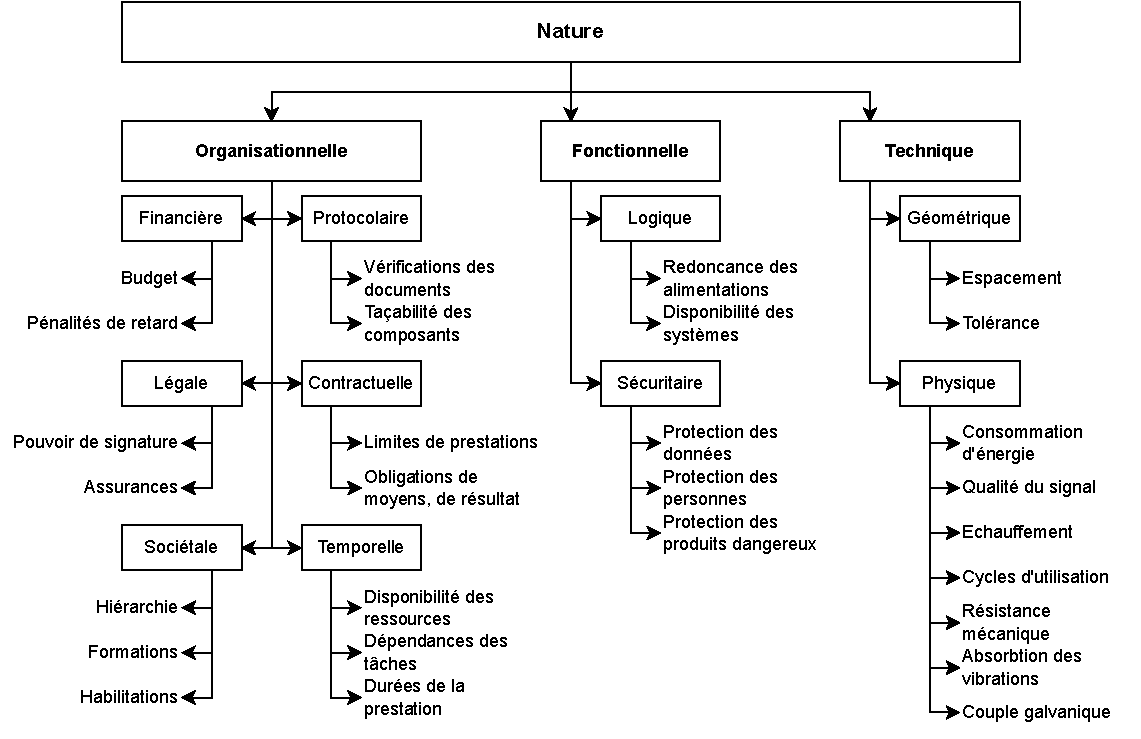
\includegraphics[width=.9\linewidth]{./svg/taxonomie.pdf}
\caption{\label{fig:org2c4d178}Hierarchie des contraintes}
\end{figure}

Justifier le besoin d'une "méthode de rédaction générique".
\subsection{Médiums et volumétrie}
\label{sec:orge67da01}
\todo[inline]{expliciter la problèmatique : taille du corpus, diversité des sources, silotage des rédactions (pas de travail conjoint entre les organismes producteurs de contraintes), difficulté d'en connaitre, etc.}
Sources, origines et finalités

Brevets, Normes, Législation, Contrats, Jurisprudences\ldots{}

Volume conséquent => faire un compte du nombre de pages par domaine pour illustrer la problématique.

\begin{figure}[htbp]
\centering
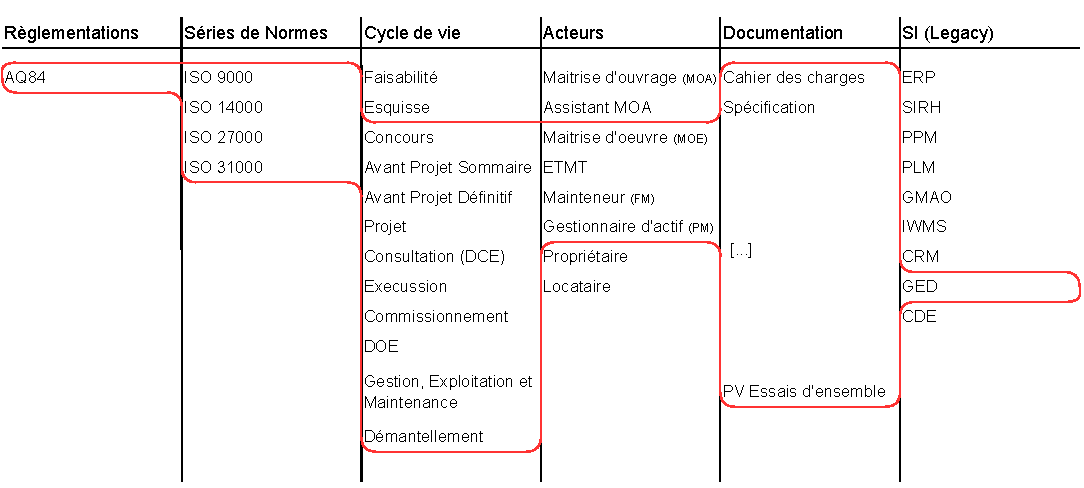
\includegraphics[width=.9\linewidth]{./svg/360-view-engineering-environment.pdf}
\caption{\label{fig:org95d5bbb}Proposition de représentation des environnements de contraintes}
\end{figure}

\todo[inline]{voie de recherche possible : création d'un service de fourniture de contrainte standardisé et unifié appelable via des requettes API}
\subsection{Exercice des contraintes}
\label{sec:orge98cbad}
\todo[inline]{expliciter le cycle de vie des contraintes}
Dans l'industrie de la construction, les parties prenantes se coordonnent dans la réponse à des exigences exprimées. Cette gestion des éxigences vise l'atteinte des objectifs du client en respect des contraintes légales, réglementaires et normatives.

\begin{quote}
Les exigences sont déterminées à partir des besoins des parties prenantes et des contraintes comme les conditions d’utilisation, les ressources et la législation. -- NF EN 60300-1:2014\autocite{GestionSureteFonctionnement2014}
\end{quote}

La relation entre éxigences et contraintes est représentée par la \ref{fig:org13b1c5b}. Ainsi, une exigence est une spécification d'un besoin tenant compte des contraintes du domaine d'étude. Cependant, la limite est souvent floue entre un besoin, une contrainte et une exigence. Les professionnels de la construction ont donc tendance à les mélanger.

\begin{figure}[htbp]
\centering
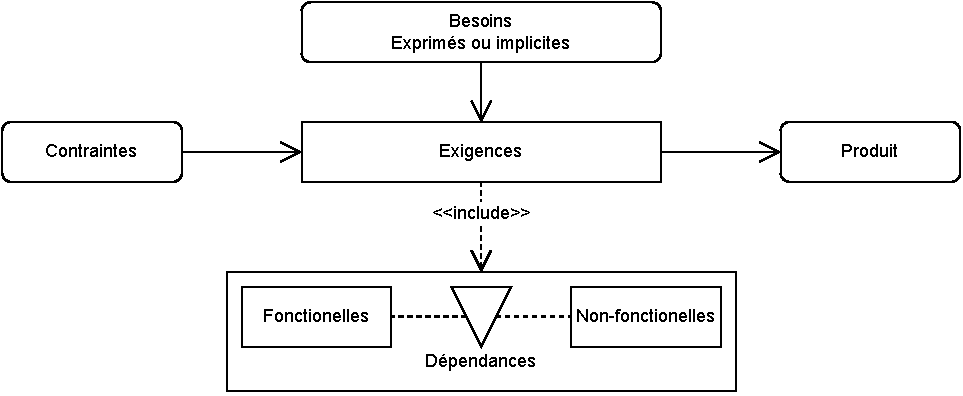
\includegraphics[width=.9\linewidth]{./svg/relation-contraintes-exigences.pdf}
\caption{\label{fig:org13b1c5b}La relation entre contraintes et exigences selont l'ISO 60300-1\autocite{GestionSureteFonctionnement2014}}
\end{figure}

Une matrice de traçabilité des exigences est employé pour réalisé le suivi des exigences.

Elle se matérialise par un tableau ou un document qui relie les exigences d'un projet aux livrables, tâches, jalons ou tests qui les satisfont. Son objectif principal est de garantir que toutes les exigences sont couvertes par les plans du projet et qu'aucun besoin n'est négligé. Elle permet également de vérifier l'impact des modifications d'exigences, facilitant la gestion des changements.

Élaboration de la matrice :
\begin{enumerate}
\item Collecte des exigences : rassembler toutes les exigences du projet, qu'elles proviennent du cahier des charges, des réunions avec les parties prenantes, d'autres documents de projet ainsi que des textes institutionnels applicables.
\item Identification des livrables : Listez tous les livrables du projet, y compris les rapports, les documents, le code source, les schémas, les maquettes numériques, les plans, etc.
\item Préparer la matrice : la première colonne source les exigences et la première ligne source les livrables. La première cellule (eg. A1:A1) est laissée vide.
\item Affecter les livrables aux exigences : Une croix est inscrite à l'intersection de chaque exigence devant être respectée ou vérifiée par un livrable. Un livrable peut être affecté à plusieurs exigences et une exigence peut nécessiter plusieurs livrables pour être vérifié. Cette étape nécessite une compréhension approfondie du projet et une collaboration étroite avec les équipes techniques.
\end{enumerate}

Utilisation de la matrice :
\begin{itemize}
\item Vérification de la couverture des exigences : la matrice permet de s'assurer que chaque exigence est adressée par au moins un livrable, réduisant ainsi le risque d'omissions.
\item Gestion des changements : Lorsque des modifications sont apportées à une exigence, la matrice facilite l'identification des livrables impactés, aidant à évaluer l'ampleur et l'impact du changement sur le projet.
\item Communication avec les parties prenantes : La matrice fournit une vue d'ensemble claire qui peut être utilisée pour communiquer l'avancement du projet et la manière dont les exigences sont satisfaites, renforçant la confiance des parties prenantes.
\item Facilitation des tests : En liant les exigences aux cas de test, la matrice aide à s'assurer que tous les aspects du système sont correctement testés, contribuant à la qualité du produit final.
\end{itemize}

La matrice de traçabilité des exigences est un document vivant qui \textbf{doit être régulièrement mis à jour tout au long du projet}. Les ajouts, les suppressions ou les modifications d'exigences, ainsi que l'évolution des plans de livrables, doivent être reflétés dans la matrice pour maintenir sa précision et sa pertinence.
Elle est employée en complément d'une liste des documents exécutés par le prestataire.

La nature de sa composition s'apparente à une table de jonction d'une base de donnée relationnelle tel que pourrait définir, sous forme de MLD la figure \ref{fig:org6ad7b5b}.

\begin{figure}[htbp]
\centering
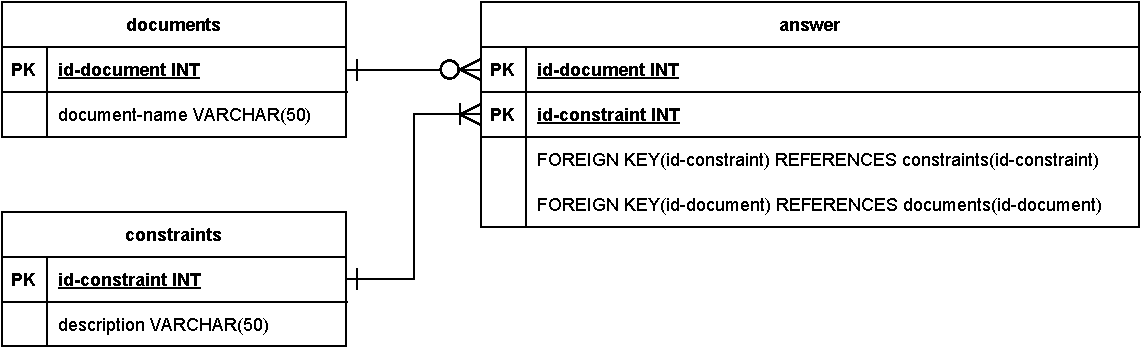
\includegraphics[width=.9\linewidth]{./svg/db-exigences-lde.pdf}
\caption{\label{fig:org6ad7b5b}MLD - Association des éxigences aux livrables}
\end{figure}
\subsection{Cadre de travail}
\label{sec:org6170e3a}
\todo[inline]{on pose ici les 3 composantes du projet de recherche lié aux contraintes}
Les contraintes étant centraux à la caractérisation d'un ouvrage, il convient de définir un cadre de travail rigoureux permettant leurs manipulation.

Ce cadre doit poséder à minimum 3 composantes :
\begin{itemize}
\item Modélisation : formulation, négociation et amélioration des contraintes ;
\item Résolution : vérification de l'espace de solution, contrôle automatisé du respect des contraintes ;
\item Préservation : suivi des évolutions, association contextuelle, recherche d'information, etc.
\end{itemize}

Modélisation des contraintes : c’est l’activité de formulation et de négociation des contraintes en amont et au fil du projet. Il s’agit d’identifier clairement toutes les contraintes pertinentes (contextuelles, contractuelles, techniques…), de les exprimer de façon non ambiguë (rédaction dans le cahier des charges, spécifications, notes de calcul, modèles \protect\hyperlink{gls-2}{\label{gls-2-use-2}UML}, etc.) et de s’assurer qu’elles sont comprises et acceptées par les parties prenantes. La modélisation inclut éventuellement la négociation de certaines contraintes : par exemple discuter d’une tolérance plus large si une exigence s’avère trop restrictive par rapport au coût, ou reformuler un besoin implicite en exigences explicites testables. Un bon modèle de contraintes se veut complet, traçable et partagé par tous, servant de référence commune.

Résolution des contraintes : ce volet recouvre la satisfaction effective des contraintes lors de la recherche de solution et de la réalisation du projet. Il s’agit d’abord de procéder à la résolution du problème en trouvant un espace de solution qui respecte l’ensemble des contraintes identifiées – en d’autres termes, vérifier qu’il existe au moins une solution faisable (vérification de la non-surcontrainte). Ensuite, on s’assure du juste niveau de contrainte : éviter d’ajouter des contraintes inutiles ou trop sévères qui surcontraindraient le projet par rapport au besoin réel. Cela implique une optimisation : assez de contraintes pour rencontrer le besoin et les objectifs, mais pas au point d’éliminer des solutions viables ou d’alourdir le projet inutilement. Enfin, ce volet inclut la vérification du respect des contraintes tout au long des études et de l’exécution – par des revues de conception, des simulations, des prototypes ou des tests. Chaque décision technique ou modification doit être évaluée au prisme des contraintes : si une solution envisagée viole une contrainte (par exemple une charge dépassant la contrainte de poids maximal), il faut soit l’ajuster, soit envisager de redéfinir la contrainte si cela est justifié et approuvé.

Préservation des contraintes (capitalisation) : au-delà du respect ponctuel, il est crucial de préserver la mémoire des contraintes du projet et de leur évolution. Ce troisième volet consiste à historiser et documenter les contraintes, leurs justifications d’origine, et les éventuelles modifications apportées en cours de route (assouplissements, ajouts, suppressions), de sorte que l’on sache à tout moment pourquoi telle contrainte a été posée et pourquoi tel choix de conception a été fait en conséquence. Cette traçabilité garantit la cohérence du projet sur la durée et facilite la maintenance ou les évolutions futures. Par exemple, conserver dans un registre ou une base de connaissance le raisonnement ayant conduit à une contrainte particulière (issue d’une norme, d’un retour d’expérience, d’une demande client spécifique…) permettra, des années plus tard, à un nouvel intervenant de comprendre le rationnel de conception. La préservation des contraintes et de leur historique de négociation contribue ainsi à une gestion de configuration rigoureuse et à l’amélioration continue du référentiel de conception de l’entreprise.

En conjuguant ces trois dimensions, on dote la notion de contrainte d’un véritable cadre de gestion sur le projet en respectant la définition \ref{org54f7041}.
\subsection{Méthodes de traitement}
\label{sec:org7d2cf3c}
Langage naturel :
\begin{itemize}
\item Rédaction
\item Affectation (par des tableaux et matrices)
\item Relecture (sur la base de listes à puces, checklist)
\item Simulations (éventuellement mais loop sur rapport produit)
\item Model checking : vérification exhaustive d'états finis, non systématique à date et loop sur rapport produit
\end{itemize}
\subsection{Conclusion}
\label{sec:orgc0fdcfe}
\clearpage
\section{Proposition}
\label{sec:org99dfd0a}
\subsection{Architecture logicielle}
\label{sec:orgfc0b4ec}
\subsubsection{Choix technologiques}
\label{sec:org2c81d9f}
\subsubsection{Modules principaux}
\label{sec:org0aa4aa4}
\subsubsection{Tests unitaires et d'intégration}
\label{sec:org1363aca}
\subsection{Conclusion}
\label{sec:orga3ea561}
\clearpage
\section{Validation expérimentale}
\label{sec:org76d5dc8}
\subsection{Protocole d'essais}
\label{sec:org1b78366}

\subsection{Cas d'étude 1 :}
\label{sec:orga3bdd66}
\subsection{Cas d'étude 2 :}
\label{sec:org84b5226}
\subsection{Cas d'étude 3 :}
\label{sec:orgb87fb27}

\subsection{Analyse comparative}
\label{sec:org631e106}
\subsubsection{Métriques de performance}
\label{sec:orge15c701}
Comment mesurerer l'efficacité ? Temps gagné ? Nombre d'erreurs détectées en amont ?
Envisager des questionnaires pour évaluer la charge mentale (ex: NASA-TLX) avant et après l'utilisation de votre outil.
\subsubsection{Limitations identifiées}
\label{sec:org0e6c7b4}
\subsection{Conclusion}
\label{sec:org890e1b2}
\clearpage
\section{Discussion et perspectives}
\label{sec:org99b72cf}
\subsection{Analyse des contributions}
\label{sec:org12562bf}
\subsubsection{Contributions théoriques}
\label{sec:orgffee61f}
\subsubsection{Contributions méthodologiques}
\label{sec:org2f7ed58}
\subsubsection{Contributions pratiques}
\label{sec:orgd382bba}
\subsection{Limites et défis}
\label{sec:orge9965d0}
\subsubsection{Limites théoriques}
\label{sec:orgbffb375}
\subsubsection{Limites pratiques}
\label{sec:orgafdf066}
\subsubsection{Défis organisationnels}
\label{sec:org6a64eaf}
\subsection{Perspectives d'amélioration}
\label{sec:orgd2f0c10}
\subsubsection{Extensions théoriques}
\label{sec:org963887d}

\begin{figure}[htbp]
\centering
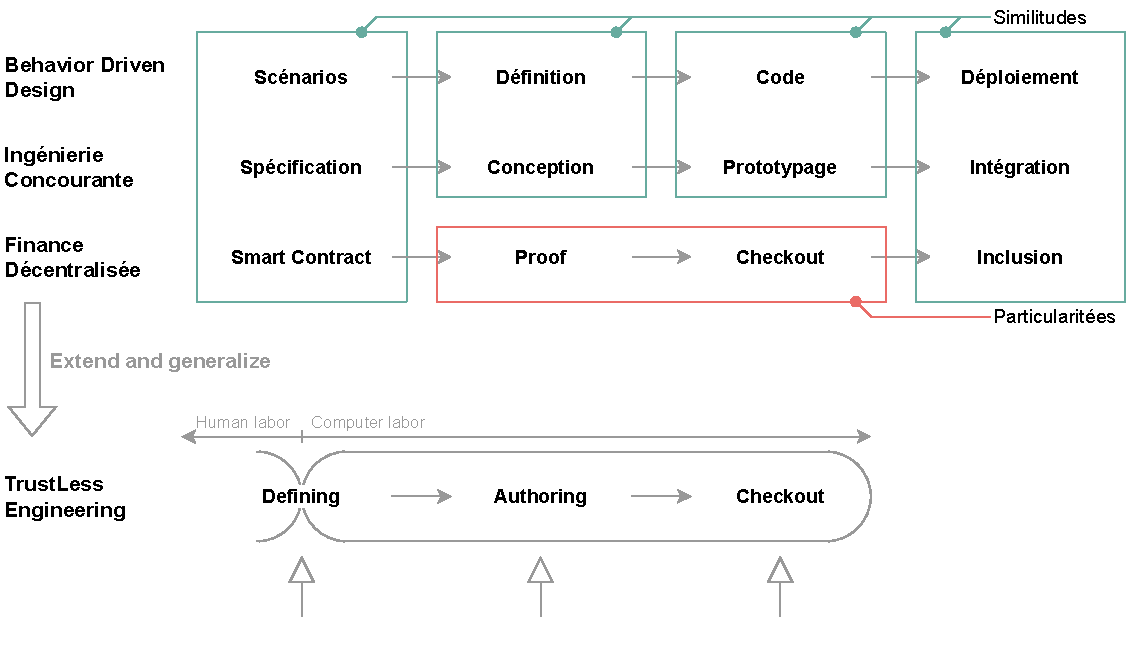
\includegraphics[width=.9\linewidth]{./svg/long-term-goal.pdf}
\caption{\label{fig:orgef31dea}Vers une ingénierie sans confiance ?}
\end{figure}
\subsubsection{Améliorations techniques}
\label{sec:orgc8ad6c2}
\subsubsection{Extensions domaines}
\label{sec:org5eb0d36}
\subsection{Impact scientifique et industriel}
\label{sec:org102ad1c}
\subsubsection{Impact sur la recherche}
\label{sec:orgd1f370d}
\subsubsection{Impact industriel}
\label{sec:orgeb80b94}
\subsubsection{Impact sociétal}
\label{sec:orga3abb6d}
Discuter de la faisabilité et des implications de la refonte de la filière.
\clearpage
\section{Conclusion générale}
\label{sec:orga7a5af7}
Synthèse des contributions

Contribution théorique majeure

Innovation méthodologique

Validation expérimentale

Réponse à la question principale

Réponse à la questions secondaires

Perspectives d'avenir


\begin{quote}
{[}!Info] Commentaire prospectif sur l'ouvrage et ses conclusions
\end{quote}

Espérer une évolution des plateformes d'accès aux normes (cobaz) pour simplifier la configuration des environnements de travail (NF EN etc. et gestion des exigences)

L'avenir, un terrain fertile pour l'ingénierie intégrée ?

Les futures ruptures technologiques (?)
\clearpage
\section{Références du document}
\label{sec:org4357a8d}
\subsection{Liste des figures}
\label{sec:org331ac87}
\renewcommand{\listfigurename}{\vspace{-2em}}
\listoffigures
\subsection{Liste des tableaux}
\label{sec:org1a992fa}
\renewcommand{\listtablename}{\vspace{-2em}}
\listoftables
\subsection{Liste des codes sources}
\label{sec:orgb06c116}
\renewcommand{\lstlistingname}{\vspace{-2em}}
\lstlistoflistings
\subsection{Liste des glosses}
\label{sec:org8c50920}


\subsection{Liste des acronymes}
\label{sec:org67d89e2}
\textbf{\hypertarget{gls-78}{BPMN}}\hspace*{1em}Business Process Model and Notation\hspace*{.5em}\pageref{gls-4-use-1}

\textbf{\hypertarget{gls-69}{BIM}}\hspace*{1em}\hspace*{.5em}\pageref{gls-1-use-1}

\textbf{\hypertarget{gls-186}{ICS}}\hspace*{1em}International Classification for Standards\hspace*{.5em}\pageref{gls-5-use-1}, \pageref{gls-5-use-2}, \pageref{gls-5-use-3}

\textbf{\hypertarget{gls-332}{SysML}}\hspace*{1em}System Model Language\hspace*{.5em}\pageref{gls-3-use-1}

\textbf{\hypertarget{gls-339}{UML}}\hspace*{1em}Unified Model Language\hspace*{.5em}\pageref{gls-2-use-1}, \pageref{gls-2-use-2}

\clearpage
\section{Bibliographie}
\label{sec:org8e74972}
\small
\printbibliography[heading=none]

\normalsize
\clearpage

\appendix
\section{Analyse des normes}
\label{sec:org3c4259b}
\subsection{Introduction}
\label{sec:orgad0dc9c}
\subsection{Périmètre de l'étude}
\label{sec:org43b3b8a}
L’étude se concentre sur les normes volontaires françaises (NF) référencées par AFNOR et publiées à la date de la collecte.
Le périmètre inclut toutes les normes relevant du domaine “Construction et urbanisme” selon la classification AFNOR Norm’Info.

Les normes ISO/IEC sont souvent transposées en normes NF (NF EN ISO, etc.)

AFNOR est le point d’entrée national reconnu par l’État pour la normalisation volontaire.

Les normes d’application obligatoire sont issues de ce corpus (via réglementations).

Par l'analyse des textes et de leurs métadonnées, nous tenterons de répondre aux questions suivantes :

\begin{itemize}
\item Q1 : Quelle est l’ampleur documentaire du corpus normatif applicable à l’industrie de la construction, mesurée en nombre de documents et en volume paginé ?
\item Q2 : La filière construction présente-t-elle une densité normative supérieure à celle d’autres secteurs industriels comparables, en termes de nombre de normes actives et de leur volumétrie documentaire ?
\item Q3 : Comment les textes normatifs se répartissent-ils entre les sous-domaines techniques, professions et spécialités représentatives de la filière construction, selon les descripteurs et indices de classement ?
\end{itemize}
\subsection{Méthodologie}
\label{sec:org44de3a1}
\subsubsection{Cadre juridique}
\label{sec:org4e2f1c1}
Il n'existe pas de base de données publiques recenssant l'ensemble des textes de normes et leurs métadonnées. Il convient donc de constituer cette base de donnée en collectant les informations publiquement accessibles.

Cette opération implique l'emplois du webscraping.

\begin{quote}
Le webscraping consiste à extraire automatiquement (to scrape : gratter), de manière massive des données d'un site web. -- INRAE\autocite{quesnevilleRecommandationsUsagesWebscraping2024}
\end{quote}

La légalité d'une telle opération semble parfois faire débat. (ref à ajouter)

Certains acteurs, notamment l'AFNOR, s'oppose à la fouille automatisée des texte que l'organisme fournis ainsi qu'à l'emploi de modèles d'intelligence artificielle sur ceux-ci tels que l'exprime ce paragraphe apposés en première page de couverture :
\begin{quote}
AFNOR, en tant que titulaire des droits d’auteur ou distributeur autorisé, s’oppose expressément à toute intégration, transmission ou absorption totale ou partielle du présent document par des moteurs ou algorithmes d’Intelligence Artificielle (IA). AFNOR s’oppose également à toute fouille de textes et de données ou création dérivée produite par une IA et basée sur le présent document.
\end{quote}

Cela dit, le Code de la propriété intellectuelle précise les modalités de copie et de reproduction des bases de données (Art. L342-3) et les droits de manipulation des textes dans un cadre de recherche scientifique (Art. L122-5 et L122-5-3)\autocite{CodeProprieteIntellectuelle} en précisant spécifiquement que :
\begin{quote}
Des copies ou reproductions numériques d'œuvres auxquelles il a été accédé de manière \textbf{licite} peuvent être réalisées \textbf{sans autorisation des auteurs} en vue de \textbf{fouilles de textes et de données} menées à bien aux seules fins de la recherche scientifique par les organismes de recherche [\ldots{}] ou pour leur compte et à leur demande par d'autres personnes, y compris dans le cadre d'un partenariat sans but lucratif avec des acteurs privés. -- Article L122-5-3\autocite{CodeProprieteIntellectuelle}
\end{quote}

L'exploration des textes publiés par l'AFNOR et obtenus de manière licite est donc autorisée.
\subsubsection{Données collectées}
\label{sec:org93facc4}
Métadonnées accessibles publiquement via Norm’Info et Boutique AFNOR :
    Référence (ex : NF C15-100)
    Titre
    Date de publication
    Nombre de pages
    Codes International Classification for Standards
 (\protect\hyperlink{gls-5}{\label{gls-5-use-1}ICS})
    Indice de classement
    Domaine technique
    Commission de normalisation
\subsubsection{Protocole technique}
\label{sec:orgd68abac}
Méthode de collecte : Web scraping (à documenter)

Limite : seules les normes publiées et publiquement référencées sur le site marchand de l'AFNOR disponibles à la vente ou référencées, sont incluses.
\subsection{Méthodes d'analyse}
\label{sec:orgcb2235f}
Analyse descriptive :
    Nombre total de documents / pages
    Évolution temporelle des publications (si date disponible)

Analyse comparative :
    Densité normative dans la construction vs autres domaines AFNOR (en comparant les volumes \protect\hyperlink{gls-5}{\label{gls-5-use-2}ICS} sectoriels)

Analyse thématique / taxonomique :
    Catégorisation des normes par code \protect\hyperlink{gls-5}{\label{gls-5-use-3}ICS}, indice de classement, domaine technique
    Projection possible par métier : architecture, génie civil, thermique, électricité…

Outils recommandés : Python (pandas + matplotlib)
\subsection{Résultats obtenus}
\label{sec:org825c82f}
Cartographie de la norme dans la construction

Poids normatif par spécialité

Identification d’une sur-normativité éventuelle

Premiers indicateurs pour évaluer la « charge de la norme »
\subsection{Discussion et perspectives}
\label{sec:org5db63a7}
\clearpage
\section{Analyse des ontologies}
\label{sec:org9763387}
Echanger avec A.Vial du CSTB pour une collaboration
Application des ontologies en gestion des contraintes
Panorama et comportement
\section{Analyse des méthodes de test logiciels}
\label{sec:orgd3fc4fd}
\section{Analyse des langages de balisage légers}
\label{sec:org5c93923}
\section{Analyse des standards d'information}
\label{sec:org9a1092e}
\clearpage
\end{document}
